\section{Metodología de la investigación}

Este estudio se desarrolló mediante una metodología de investigación aplicada con
evaluación experimental. El problema abordado exigió diseñar, implementar y
validar una estrategia de compresión sin pérdida de precisión sobre un simulador
cuántico tipo Schrödinger, manteniendo la exactitud numérica del estado y
cuantificando el efecto de la compresión sobre memoria y tiempo. En consecuencia,
la metodología combinó revisión del estado del arte, selección justificada de
herramientas, diseño de la arquitectura de almacenamiento, integración en el
simulador base y experimentación controlada sobre cargas de trabajo
representativas.

\begin{figure}[H]
    \centering
    \caption{Metodología de investigación}
    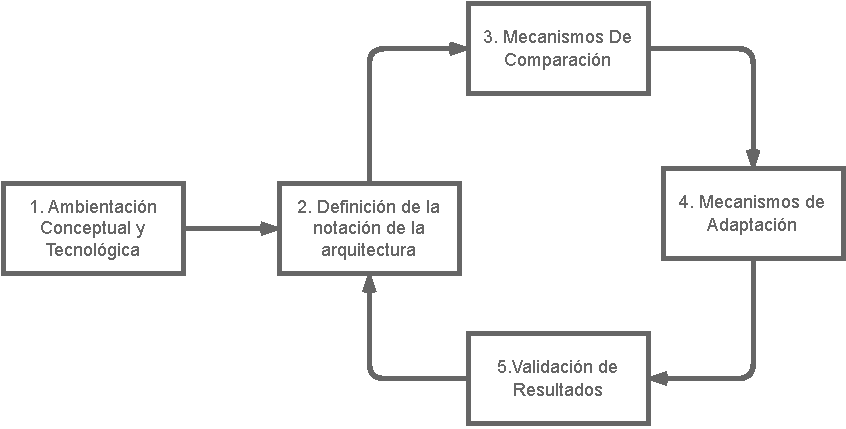
\includegraphics[width=0.7\linewidth]{images/Metodologia.pdf}
    \label{fig:met}
\end{figure}



\subsection{\normalsize Diseño}
Comprendió el estudio del estado del arte, la definición de requisitos y supuestos, la selección del simulador y la planificación experimental y de integración técnica.

\begin{itemize}
  \item \textbf{Revisión de literatura y estado del arte.} Se realizó una revisión estructurada de técnicas de compresión sin pérdida de precisión para arreglos de punto flotante y de su aplicabilidad en simulación cuántica de \emph{vectores de estado}. A partir de esa revisión se identificaron ventajas, limitaciones y brechas relevantes para el problema.
  \item \textbf{Criterios y procedimiento de selección del simulador cuántico.} Se evaluaron alternativas como QuEST, Intel-QS, qsim, Quantum++ y TMFQSfullstate con base en apertura y modificabilidad del código, facilidad de integración de estructuras personalizadas para el vector de estado, soporte a optimizaciones de memoria y paralelismo, y capacidad de instrumentación de tiempo y memoria. La decisión se formalizó mediante una matriz ponderada.
  \item \textbf{Arquitectura de la solución y diseño de la estrategia de compresión.} Se definieron las estructuras de datos y los puntos de inserción en la capa de almacenamiento del vector de amplitudes, junto con las políticas de compresión, descompresión y reutilización temporal de bloques requeridas por la integración.
\end{itemize}

\subsection{\normalsize Implementación e integración de la estrategia}
La estrategia de compresión seleccionada se implementó en el simulador cuántico
elegido, modificando su sistema de almacenamiento y gestión de memoria. Durante
esta etapa se optimizó el esquema de acceso para evitar sobrecostos
computacionales innecesarios asociados a la compresión y descompresión. Las
actividades principales fueron las siguientes:
\begin{itemize}
    \item Modificación del código fuente del simulador para integrar la compresión
        sin pérdida.

    \item Optimización del sistema de almacenamiento para reducir el uso de memoria
        y controlar la sobrecarga temporal.

    \item Validación inicial de la implementación mediante circuitos de prueba y
        comprobación de igualdad exacta frente a la referencia no comprimida.
\end{itemize}
\subsection{\normalsize Evaluación experimental}
Se diseñó una campaña experimental para evaluar el impacto de la estrategia de
compresión sobre circuitos cuánticos con estructuras de estado contrastantes. La
evaluación permitió determinar en qué condiciones la compresión sin pérdida
ofrece un balance favorable entre ahorro de memoria y costo temporal. En esta
fase se realizaron las siguientes actividades:
\begin{itemize}
    \item Definición de un conjunto de circuitos de prueba para evaluar la estrategia
        de compresión:
        \begin{itemize}
            \item Transformada de Fourier Cuántica (QFT)

            \item Algoritmo de búsqueda de Grover
        \end{itemize}

    \item Ejecución de simulaciones con y sin compresión para medir su impacto en
        el rendimiento y el uso de memoria:
        \begin{itemize}
            \item Tiempo de ejecución total (segundos)

            \item Uso máximo de memoria (MB)

            \item Verificación de igualdad exacta del estado respecto a la referencia sin compresión:
                \[
        \alpha_i^{(\text{ref})} = \alpha_i^{(\text{comp})} \quad \forall i.
      \]

            \item Error absoluto máximo como medida auxiliar de discrepancia:
                \[
        e_{\text{abs}} = \max_i \left|\alpha_i^{(\text{ref})} - \alpha_i^{(\text{comp})}\right|.
      \]
        \end{itemize}

    \item Análisis de los resultados obtenidos y contraste con el almacenamiento no
        comprimido y con una estrategia complementaria de compresión con pérdida
        controlada.
\end{itemize}

La campaña experimental se ejecutó sobre la estación de trabajo donde se desarrolló el simulador, equipada con Rocky Linux 10.1, procesador AMD Ryzen 7 5700X de 8 núcleos y 16 hilos, y 32~GiB de memoria RAM. Las métricas de tiempo y memoria residente máxima se recolectaron con \texttt{psrecord} a partir de las ejecuciones de los binarios experimentales del simulador. En Grover se promediaron tres instancias por tamaño para reducir la dependencia de la posición de los estados marcados; en los registros empleados, la dispersión temporal entre esas tres posiciones se mantuvo acotada y la memoria pico permaneció prácticamente invariante para una misma estrategia y un mismo tamaño. En QFT se reportó una instancia por familia de entrada y por número de qubits.

La verificación de exactitud para la estrategia sin pérdida se realizó exportando el vector completo de amplitudes de la ejecución de referencia no comprimida y el vector completo de la ejecución con almacenamiento Blosc sobre la misma carga de trabajo, para luego compararlos amplitud por amplitud. En la estrategia con pérdida basada en ZFP, el error reportado se obtuvo mediante el mismo procedimiento de exportación completa, resumiendo la discrepancia con el máximo error absoluto frente a la referencia no comprimida.
